\section{Several manoeuvres}\label{sec:several}

\subsection{The escape length}
For a configuration $q$ with left centre $C$ satisfying $|C_y-H|\le\rho$, define the \emph{escape length}
\[
  V(q)=C_x+\sqrt{\rho^2-(C_y-H)^2}.
\]
It is the abscissa at which the front curb-side corner would cross the height $H$ if the car drove forward with full left lock from $q$.
The proof of \cref{prop:one-forward} shows that (under \cref{ass:one}) a forward exit from a parked configuration $q$ requires $L\ge V(q)$; heuristically the same holds for low, nearly level configurations.
Conversely, $V(q)\le L$ suffices when the curb and the rear are not in the way.
By \cref{lem:drift}, $C$ moves only along $\pm\e(\psi)$, which yields the following bookkeeping:
\begin{itemize}[nosep]
\item forward or reverse \emph{full left lock} leaves $C$, and hence $V$, unchanged;
\item reverse motion moves $C$ backwards, so $V$ decreases (as long as $\psi$ is moderate), fastest under full right lock, where $C$ moves at speed $2$;
\item forward motion without full left lock moves $C$ forwards and increases $V$.
\end{itemize}
A good multi-manoeuvre exit therefore alternates two kinds of manoeuvre.
Reverse arcs with full right lock lower $V$ and turn the car nose-up.
Forward arcs with full left lock keep $V$ fixed, create room behind the car and also turn it nose-up.
The reverse arcs are limited by the curb and by the car behind, the forward arcs by the car in front.
The final manoeuvre is a forward full-left-lock exit, possible once $V\le L$.

\subsection{Two manoeuvres}

\begin{proposition}\label{prop:two}
Let $\alpha\in(0,\pi/2)$ be the solution of
\begin{equation}\label{eq:alpha2}
  \Rm(1-\cos\alpha)+d_b\sin\alpha=m ,
\end{equation}
and put
\[
  \Lambda_2=d_b\cos\alpha-\Rm\sin\alpha+\sqrt{\rho^2-(2R\cos\alpha-\Rp)^2}.
\]
Assume $\Rm+d_b>m$, $d_b<b$, $\alpha\ge\beta$, $d_b\cos\alpha\ge\Rm\sin\alpha$, $r\cos(\alpha-\beta)-d_b\ge H$, $d_b\cos\alpha+\Rp\sin\alpha+b\le\Lambda_2$, $\max(b,d_b)\tan\alpha<\Rm$ and $\Rp\ge d_b\tan(\alpha/2)$.
Then $\Lmin(2)\le\Lambda_2$.
\end{proposition}

The left-hand side of \eqref{eq:alpha2} increases from $0$ to $\Rm+d_b>m$ on $[0,\pi/2]$, so $\alpha$ is well defined.
(The inequality $2R\cos\alpha\ge\Rp$ used below follows from $C_{1,y}=r\cos(\alpha-\beta)\ge H+d_b$.)
For the typical car, $\alpha=0.1732$ rad $=9.93^\circ$, $\beta=0.1717$ rad and $\Lambda_2=5.4247$~m, and all hypotheses hold; the thinnest margin is $\alpha-\beta=0.0015$ rad.
The two-manoeuvre gap is thus $0.41$ m shorter than the one-manoeuvre gap.

\begin{proof}
We describe an exit with $L=\Lambda_2$; see \cref{fig:two}.
Let $x_0=d_b\cos\alpha+\Rp\sin\alpha$ and start from the level configuration $q_0=((x_0,m+\tfrac w2),0)$.
It is parked: its footprint is $[x_0-d_b,x_0+b]\times[m,H]$, with $x_0-d_b=\sin\alpha\,(\Rp-d_b\tan\frac\alpha2)\ge0$ and $x_0+b\le L$ by assumption.

\emph{Manoeuvre 1: reverse with full right lock through the angle $\alpha$.}
The car rotates counter-clockwise about the fixed right centre $C'=(x_0,m+\tfrac w2-R)$.
After rotating by $t\in[0,\alpha]$, a body point $(u,v)$ sits at $C'$ plus the vector $(u,v+R)$ rotated by $t$.
That vector has vertical component $u\sin t+(v+R)\cos t\ge\Rm\cos t-d_b\sin t>0$, because $d_b\tan\alpha<\Rm$.
So every point stays above $C'$ and moves to the left. Moreover:
\begin{itemize}[nosep]
\item the leftmost point $\cRL$ has $x=x_0-d_b\cos t-\Rp\sin t\ge0$, with equality at $t=\alpha$, so the car never enters $\Or$;
\item the lowest point $\cRC$ has height $m-\Rm(1-\cos t)-d_b\sin t\ge0$, with equality at $t=\alpha$; its abscissa $x_0-d_b\cos t-\Rm\sin t$ decreases in $t$ and ends at $w\sin\alpha\ge0$;
\item the front moves away from $\Of$.
\end{itemize}
At the end, $q_1=(P_1,\alpha)$ with $P_1=C'+R(-\sin\alpha,\cos\alpha)$.
Both rear corners are in contact: $\cRC$ with the curb and $\cRL$ with the car behind.
The left centre of $q_1$ is
\[
  C_1=\big(x_0-2R\sin\alpha,\ m+\tfrac w2-R+2R\cos\alpha\big)=\big(d_b\cos\alpha-\Rm\sin\alpha,\ H+2R\cos\alpha-\Rp\big).
\]

\emph{Manoeuvre 2: forward with full left lock to heading $\pi/2$, then full right lock to heading $0$.}
We follow the proof of \cref{prop:one-upper} with $C_1$ in place of $C$.
\begin{itemize}[nosep]
\item By the choice of $L$, $|C_1-\Qf|=\rho$; also $C_{1,x}\le L$ and $C_{1,y}\ge H$, so $\Of$ misses the disk of radius $\rho$ about $C_1$.
\item Every point of the car is below $C_1$: the highest point $\cFL$ lies below $C_1$ by $\Rm\cos\alpha-b\sin\alpha>0$. Since also $C_{1,x}\ge0$, no point enters $\Or$ (polar-angle argument).
\item For the curb: by \eqref{eq:RCy}, $0=\cRC_y(q_1)=C_{1,y}-r\cos(\alpha-\beta)$.
Since $\alpha\ge\beta$, $\cRC$ has already passed the bottom of its circle and now rises.
The points that still pass through the bottom of their circles have body coordinates with $u<-(R-v)\tan\alpha$.
Their distance from $C_1$ is less than $|u|/\sin\alpha\le d_b/\sin\alpha$.
Since $\sin\alpha\cos(\alpha-\beta)-\sin\beta=\tfrac12\big(\sin(2\alpha-\beta)-\sin\beta\big)\ge0$ for $\beta\le\alpha\le\pi/2$, we get $d_b/\sin\alpha\le r\cos(\alpha-\beta)=C_{1,y}$.
Hence these points stay above the curb.
\item At heading $\pi/2$ the lowest point has height $C_{1,y}-d_b=r\cos(\alpha-\beta)-d_b\ge H$, and the final right-lock arc keeps the car in the lane as in \cref{prop:one-upper}.
\end{itemize}
This is a free exit with two manoeuvres; \cref{lem:reversal} turns it into a parking motion.
\end{proof}

In driving terms (forward time) the strategy is the familiar one.
Reverse in along an S-curve (right lock, then left lock) and stop when the car, turned $\alpha\approx10^\circ$ nose-up, touches the curb with its rear corner and the car behind with its rear bumper.
Then pull forward with full right lock until the car is level.

\begin{figure}[ht]
\centering
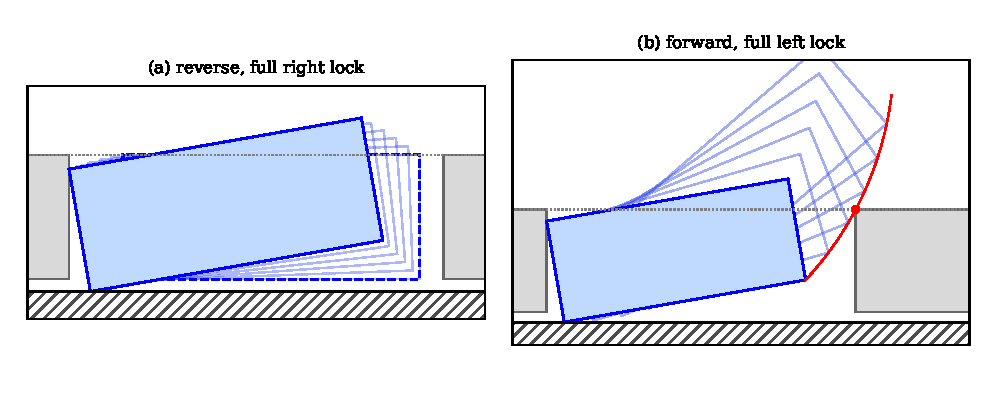
\includegraphics[width=\textwidth]{figures/fig_two.pdf}
\caption{The two-manoeuvre exit of \cref{prop:two} for the typical car ($L=\Lambda_2$).
(a) Reverse with full right lock from the level position (dashed) until both rear corners touch.
(b) Forward exit with full left lock; the front curb-side corner (red) grazes $\Qf$.}
\label{fig:two}
\end{figure}

\begin{remark}\label{rem:two-other}
If $\alpha<\beta$, stopping the reversal at the double contact would make the rear corner dip into the curb during the exit.
One then stops the reversal at the angle $\alpha_d\le\alpha$ given by $2R\cos\alpha_d=r+\Rp-H$, so that $C_{1,y}=r$, and chooses $x_0=d_b\cos\alpha_d+\Rp\sin\alpha_d$; the angle exists when $r+\Rp-H\le2R$, i.e.\ when $m\ge\varepsilon_b$.
This gives $\Lmin(2)\le d_b\cos\alpha_d-\Rm\sin\alpha_d+\sqrt{\rho^2-(r-H)^2}$, provided the analogues of the hypotheses of \cref{prop:two} hold at $\alpha_d$: $X(\alpha_d)\ge0$, $r-d_b\ge H$, $x_0+b\le L$, $\max(b,d_b)\tan\alpha_d<\Rm$ and $\Rp\ge d_b\tan(\alpha_d/2)$.
The proof is that of \cref{prop:two}, except that the curb step of the exit is now the argument of \cref{prop:one-upper}: $C_{1,y}=r$, and the points that pass the bottom of their circles are at distance at most $r$ from $C_1$.
\end{remark}

\subsection{A better two-manoeuvre exit}\label{sec:two-better}

\Cref{prop:two} does not use the room in front of the car.
Starting further forward and first reversing briefly with \emph{left} lock tilts the car nose-down by a small angle $a_0$.
The subsequent right-lock arc then runs from $-a_0$ to a slightly larger final tilt $\alpha_1>\alpha$.
The left centre drops by about the same amount as in \cref{prop:two}, because in both cases the curb contact pins $C_{1,y}$ near $r$, but it moves back further: $2R(\sin a_0+\sin\alpha_1)$ instead of $2R\sin\alpha$.
With the larger final tilt this gives a smaller $C_{1,x}=X(\alpha_1)$, and hence a shorter slot.
The optimal choice makes three contacts: the front bumper with the car in front at the start, and, at the end of the reverse manoeuvre, the two rear corners with the curb and with the car behind.

\begin{proposition}\label{prop:two-better}
Suppose that $\alpha_1\in[\beta,\pi/2)$ and $a_0\in(0,\pi/2)$ solve
\begin{align}
  2R\cos a_0&=H+\Rm(1+\cos\alpha_1)-d_b\sin\alpha_1, \label{eq:tc1}\\
  b+2R(\sin a_0+\sin\alpha_1)&=\sqrt{\rho^2-\big(r\cos(\alpha_1-\beta)-H\big)^2}, \label{eq:tc2}
\end{align}
and put $\Lambda_2^*=b+2R\sin a_0+d_b\cos\alpha_1+\Rp\sin\alpha_1$.
Assume in addition $d_b<b$, $\gamma+a_0\le\pi/2$, $H+\Rm\ge\rho\sin(\gamma+a_0)$, $d_b\cos\alpha_1\ge\Rm\sin\alpha_1$, $r\cos(\alpha_1-\beta)-d_b\ge H$, $\Rp\ge d_b\tan(\alpha_1/2)$, and
\[
  \max(b,d_b)\tan a_0<\Rm,\qquad \Rm\tan a_0<d_b,\qquad \max(b,d_b)\tan\alpha_1<\Rm .
\]
Then $\Lmin(2)\le\Lambda_2^*$.
\end{proposition}

For the typical car, $a_0=0.04116$ rad, $\alpha_1=0.17815$ rad and $\Lambda_2^*=5.4104$ m.
This improves on $\Lambda_2=5.4247$.

\begin{proof}
Let $L=\Lambda_2^*$ and start from the level configuration with $P_0=(L-b,\,m+\tfrac w2)$.
It is parked, and its front bumper touches the car in front.

\emph{Reverse with full left lock by $a_0$.}
This is a clockwise rotation about the left centre $C_0=(L-b,\,H+\Rm)$.
The car stays below $C_0$ throughout, since its highest corner $\cRL$ lies below $C_0$ by $\Rm\cos\psi-d_b|\sin\psi|>0$ (because $d_b\tan a_0<\Rm$).
Hence all points have negative $x$-velocity, and the car moves away from the car in front.
The lowest point is $\cFC$, at height $C_{0,y}+\rho\sin(\psi-\gamma)$, which decreases to $C_{0,y}-\rho\sin(\gamma+a_0)\ge0$ by assumption.
The rear rises.
For heading $\psi\in[-a_0,0]$ the leftmost corner is $\cRC=C_0+r\,\e(\psi-\frac\pi2-\beta)$, with abscissa $C_{0,x}-d_b\cos\psi-\Rp|\sin\psi|\ge L-\ell-\Rp\sin a_0$.
By the definition of $\Lambda_2^*$,
\[
  L-\ell=2R\sin a_0+\sin\alpha_1\big(\Rp-d_b\tan\tfrac{\alpha_1}2\big)\ \ge\ 2R\sin a_0\ \ge\ \Rp\sin a_0 .
\]
Hence the car stays clear of $\Or$.

\emph{Reverse with full right lock from heading $-a_0$ to $\alpha_1$.}
This is a counter-clockwise rotation about the right centre
\[
  C'_a=C_0-2R\big(\sin a_0,\cos a_0\big)=\big(L-b-2R\sin a_0,\ H+\Rm-2R\cos a_0\big).
\]
A body point has position $C'_a$ plus the vector $(u,v+R)$ rotated by $\psi$; its vertical component relative to $C'_a$ is $u\sin\psi+(v+R)\cos\psi\ge\Rm\cos\psi-\max(b,d_b)|\sin\psi|>0$ for $\psi\in[-a_0,\alpha_1]$.
So every point stays above $C'_a$ and moves left.
Relative to $C'_a$ the corners $\cRC$ and $\cRL$ have body coordinates $(-d_b,\Rm)$ and $(-d_b,\Rp)$.
Hence
\[
  \cRC_y=C'_{a,y}-d_b\sin\psi+\Rm\cos\psi,\qquad \cRL_x=C'_{a,x}-d_b\cos\psi-\Rp\sin\psi .
\]
Both are strictly decreasing for $\psi\in[-a_0,\alpha_1]$.
For $\cRC_y$ the derivative $-d_b\cos\psi-\Rm\sin\psi$ is negative because $\tan a_0<d_b/\Rm$.
For $\cRL_x$ the derivative $d_b\sin\psi-\Rp\cos\psi$ is negative because $\tan\alpha_1<\Rm/d_b<\Rp/d_b$.
By \eqref{eq:tc1}, $\cRC_y=0$ exactly at $\psi=\alpha_1$; by the definition of $\Lambda_2^*$, $\cRL_x=0$ exactly at $\psi=\alpha_1$.
So both contacts occur only at the end.
While $\psi<0$ the lowest point is $\cFC$; it lies to the right of $C'_a$ and therefore rises.
The leftmost corner is then $\cRC$, with abscissa $C'_{a,x}-d_b\cos\psi+\Rm|\sin\psi|\ge C'_{a,x}-d_b=L-\ell-2R\sin a_0\ge0$.
The front moves away from $\Of$.

\emph{Forward exit.}
Composing the two rotations, the left centre at heading $\alpha_1$ is $C_1=C'_a+2R\,\n(\alpha_1)$.
By the definition of $\Lambda_2^*$ and by \eqref{eq:tc1}, this gives
\[
  C_1=\big(d_b\cos\alpha_1-\Rm\sin\alpha_1,\ \Rp\cos\alpha_1+d_b\sin\alpha_1\big)=\big(d_b\cos\alpha_1-\Rm\sin\alpha_1,\ r\cos(\alpha_1-\beta)\big).
\]
Equation \eqref{eq:tc2} is equivalent to $|C_1-\Qf|=\rho$.
The rest of the argument is the proof of \cref{prop:two} verbatim, with $\alpha_1$ in place of $\alpha$.
\end{proof}

In forward time the second manoeuvre pulls forward with full right lock until the car points slightly nose-down, then with full left lock until it is level and touches the car in front.

\subsection{Three or more manoeuvres}\label{sec:zigzag}

For $n\ge3$ we use \emph{rotation zigzags}.
The exit alternates forward full-left-lock arcs and reverse manoeuvres, ending with the forward escape.
A reverse manoeuvre is a full-right-lock arc, possibly preceded by a short full-left-lock arc (of at most $0.1$ rad), as in \cref{prop:two-better}.
For odd $n$ it starts with a forward arc, for even $n$ with a reverse arc.
The free parameters are the starting position and the length of each arc as a fraction of the maximal collision-free length.
We optimised them numerically for the typical car (\cref{app:numerics}); \cref{tab:zigzag} lists the results.
The car turns further nose-up at every manoeuvre and gains clearance from the curb, which in turn permits a longer next reverse arc.

\begin{table}[ht]
\centering
\begin{tabular}{lcccccc}
\toprule
$n$ & 1 & 2 & 3 & 4 & 5 & 6\\
\midrule
upper bound for $\Lmin(n)$ [m] & 5.833 & 5.411 & 5.280 & 5.180 & 5.050 & 4.978\\
\bottomrule
\end{tabular}
\caption{Best rotation-zigzag strategies found for the typical car ($n=1$ exact, $n=2$ from \cref{prop:two-better}; the search for $n=6$ was stopped early). Upper bounds are rounded up.}
\label{tab:zigzag}
\end{table}

\Cref{fig:values} compares these values with the crawl of \cref{sec:asym}.
\Cref{app:five,app:twenty} show a five- and a twenty-manoeuvre parking motion in detail, and \cref{app:cars} gives values for other cars.

How far can rotation alone go?
In the \emph{greedy} zigzag every arc is driven until contact, and the car escapes as soon as $V\le L$.
For the typical car it needs $2,3,4,8,14$ manoeuvres for slack $g=1.3,1.1,0.9,0.7,0.6$ m respectively.
For $g\le0.5$ m it stalls: the car stops turning before it can escape.

\begin{figure}[ht]
\centering
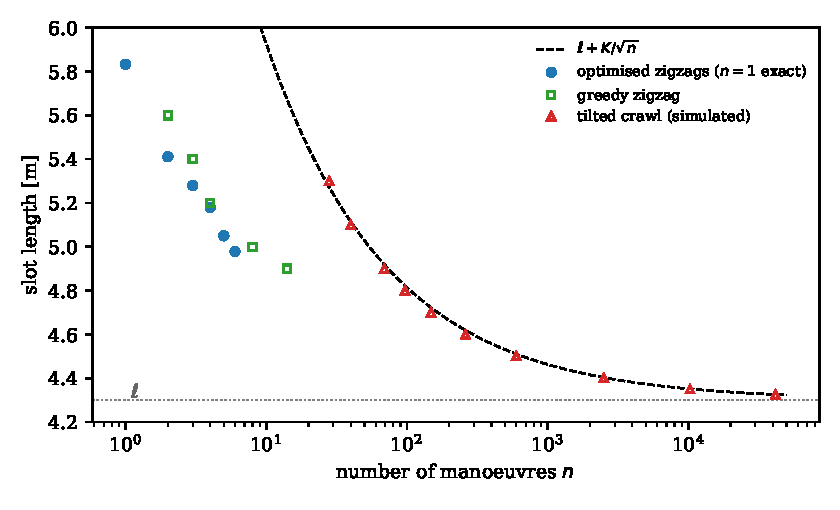
\includegraphics[width=0.8\textwidth]{figures/fig_values.pdf}
\caption{Slot lengths achieved with $n$ manoeuvres for the typical car.
All points are upper bounds for $\Lmin(n)$, except $n=1$, which is exact.
Filled circles: optimised rotation zigzags; squares: greedy zigzags; triangles: simulated tilted crawls.
The dashed curve is the sharp asymptotics $\ell+K/\sqrt n$ of \cref{thm:asym}.
Rotation is far more efficient for few manoeuvres; the crawl is asymptotically optimal.}
\label{fig:values}
\end{figure}

For large $n$ the rotation mechanism is exhausted.
Once the gap is only slightly longer than the car, every exit stays nearly level until the car has almost left the slot (\cref{lem:confine}).
Progress then comes from lateral \emph{crawling}, analysed in \cref{sec:asym}.

\begin{conjecture}\label{conj:two}
For the typical car, $\Lmin(2)=\Lambda_2^*$.
\end{conjecture}

The evidence is numerical.
We ran differential-evolution searches over exits consisting of a reverse manoeuvre followed by a forward full-left-lock escape.
The reverse manoeuvre was made of up to three arcs of arbitrary curvature and length, with arbitrary starting position, height and tilt.
Exits that begin with a forward manoeuvre end in reverse and were not searched.
At $L=5.40$ m they found no feasible two-manoeuvre exit.
The searches over left-then-right full-lock reverse arcs converge to the triple contact of \cref{prop:two-better}.
A proof would need a calibration adapted to the three contact constraints, in the spirit of \cref{sec:asym}.
